\chapter{Results} \label{results}

The wireless stethoscope exhibited unstable feedback when using it with a nearby speaker. To determine if this feedback was electrical in nature we measured the frequency response of the amplification and input circuitry stage to look for any resonant frequencies. We also measured the sound characteristics of the stethoscope tube to characterise the sound that doctor's listen to through the stethoscope. In addition we analysed auscultation recordings to find what frequency range most stethoscope sounds occur, so that future designs may utilise a lower sampling rate. 

\section{Unstable Feedback} \label{feedback-freq}
When we used the wireless stethoscope with a Blue tooth speaker within 5m near the stethoscope head the system experienced unstable feedback. This happened within a few seconds of turning the stethoscope on, a loud screech developed in the system and it became unusable. This screech is a result of feedback from the speaker into the microphone sensor. By placing the stethoscope head close to the speaker and taking an FFT of the resulting uncontrolled feedback signal, we characterised at which frequencies the feedback occurred. This frequency depended on how the microphone was coupled to the stethoscope head. When using a 3D printed cone approximately 3cm long  the dominant feedback frequency was 916Hz (Fig~\ref{fig:feedback_cone}). Higher order multiples of this fundamental 916Hz frequency also occurred in the unstable feedback, at 1820Hz, 2760Hz, 3600Hz etc. When using a short length of the original stethoscope tube to couple the microphone to the stethoscope head the dominant unstable frequency shifted from 916Hz to 1950Hz, and higher order multiples at 3900Hz, 5910Hz etc (Fig~\ref{fig:feedback_tube}). To make the device functional we had to filter out these undesired unstable feedback frequencies.

\begin{figure}[!tbh]
	\centering
	 % \fbox{
		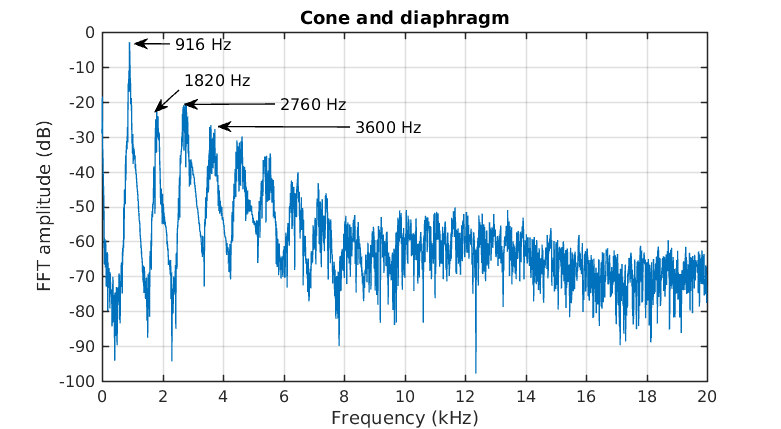
\includegraphics[width=140mm]{result_feedback_spectrum_cone.png}
	 % }
	\caption{Spectrum of feedback noise when using 3D printed cone to couple microphone to stethoscope head}
	\label{fig:feedback_cone}
\end{figure}

\begin{figure}[!tbh]
	\centering
	 % \fbox{
		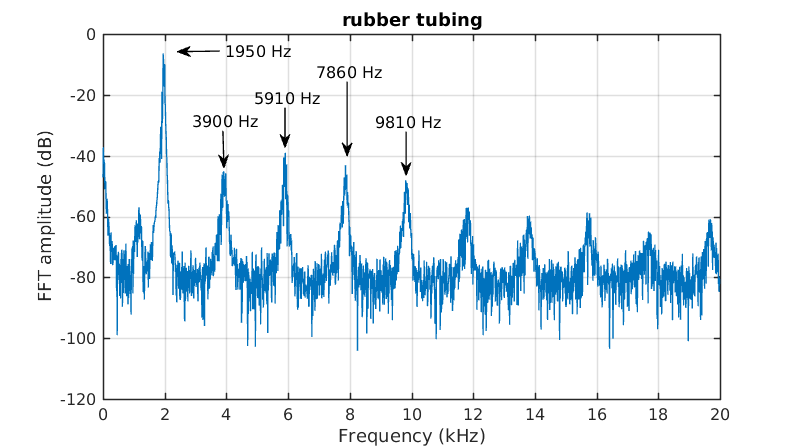
\includegraphics[width=140mm]{result_feedback_spectrum_tube.png}
	 % }
	\caption{Spectrum of feedback noise when using stethoscope tube to couple microphone to stethoscope head}
	\label{fig:feedback_tube}
\end{figure}

To prevent unstable feedback we introduced a notch filter into the system to block out the fundamental frequency (Fig.~\ref{fig:notch_circuit}). We tested the system with a notch filter placed between the low pass filter and non-inverting amplifiers. We used the 3D printed cone to couple the microphone to the stethoscope, so the notch filter was designed to stop 920Hz (Fig~\ref{fig:notch_sim}). With the notch filter in place the system no longer exhibited unstable feedback when the stethoscope was placed 5m from the Blue-tooth speaker, however unstable feedback did occur however when the stethoscope was placed within approximately 10cm of the speaker. 

\begin{figure}[!tbh]
	\centering
	 \fbox{
		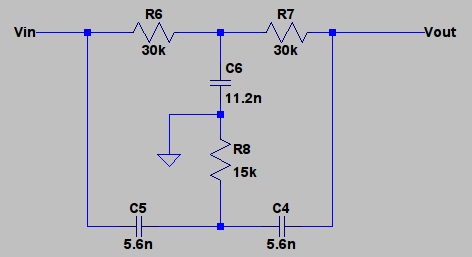
\includegraphics[width=90mm]{twinT_notch_circuit.png}
	 }
	\caption{Twin-T notch circuit used to filter out 920Hz feedback signal, taken from Horowitz\cite[p.~279]{Horowitz1989}}
	\label{fig:notch_circuit}
\end{figure}

\begin{figure}[!htb]
	\centering
	 % \fbox{
		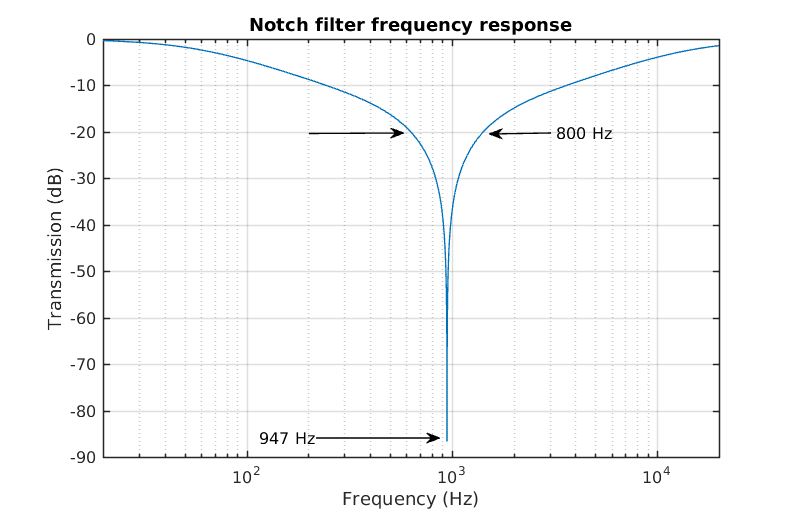
\includegraphics[width=125mm]{notch_filter_freq_response.png}
	 % }
	\caption{Simulated frequency response of twin-T notch filter}
	\label{fig:notch_sim}
\end{figure}


\section{Electrical Frequency Response}
To help identify the cause of the unstable feedback we measured the frequency response of the Signal Amplification and Input Circuitry stage of the stethoscope (Fig.~\ref{fig:sys_overview}). We measured the frequency response by placing a 10mV peak-peak signal at the input of the of the instrumentation amplifier, and recording the amplitude of the output signal at the clipping circuit. We calculated transmission as the ratio of the output signal amplitude to the input signal amplitude. In order to take transmission data for many frequencies we automated the measurements on the Agilent 3014A Mixed Signal Oscilloscope using the Standard Commands for Programmable Instruments (SCPI) interface and a simple Python script (see Appendix). We found that the electrical circuit did not exhibit any resonant frequencies about the unstable frequency 920Hz, and closely resembled the simulated transmission calculated using LTSpice (Fig~\ref{fig:result_circuit_freq_response}).

\begin{figure}[!htb]
	\centering
	 % \fbox{
		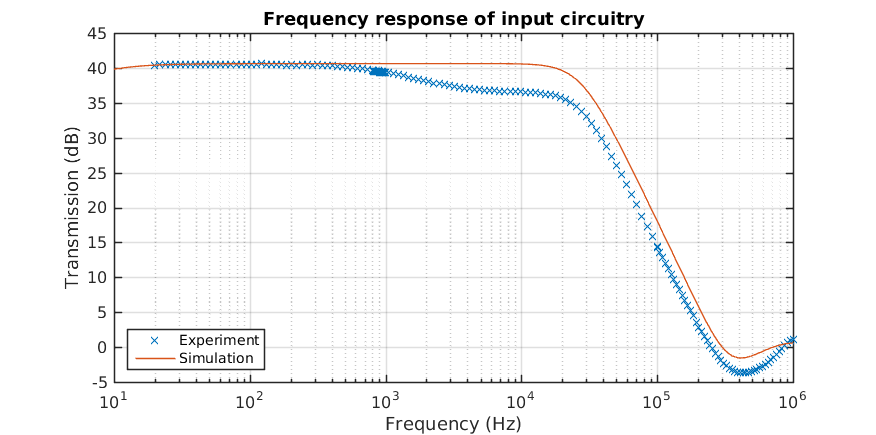
\includegraphics[width=140mm]{result_freq_response.png}
	 % }
	\caption{Frequency response of signal amplification and input circuitry stage}
	\label{fig:result_circuit_freq_response}
\end{figure}


\section{Stethoscope Acoustic Properties}
To characterise the acoustic properties of a conventional stethoscope we measured the sound frequency response of the tubing. This is because a major difference with our stethoscope design is that there is no long tubing from the head to the ear piece, only a short length of tube used to couple the microphone as close to the diaphragm as possible. This could potentially introduce a difference in sound qualities, which need to be measured in order to be compensated for.

To measure the frequency response of a headphone speaker was placed inside one end of the stethoscope tube, with the head removed. A microphone was placed at the ear piece to measure the output sound signal amplitude, then the tubing was removed and the microphone was placed right next to the speaker to get an input signal amplitude. The amplitude of the input and output signals was taken by fitting a sinusoid that minimised the sum of squared errors, and the transfer function was taken as the ratio of the two amplitudes. 

We found that there were several resonant frequencies of the tubing below 2kHz, with a dominant resonance at 850-950Hz (Fig.~\ref{fig:result_tubing_freq_response}) (Note this is unrelated to the unstable feedback frequency). The tube has a complicated transfer function but tends attenuate frequencies above 6kHz most. In order to implement a digital filter that resembles this transfer characteristic we predict we'd need a high order filter.

\begin{figure}[!htb]
	\centering
	 % \fbox{
		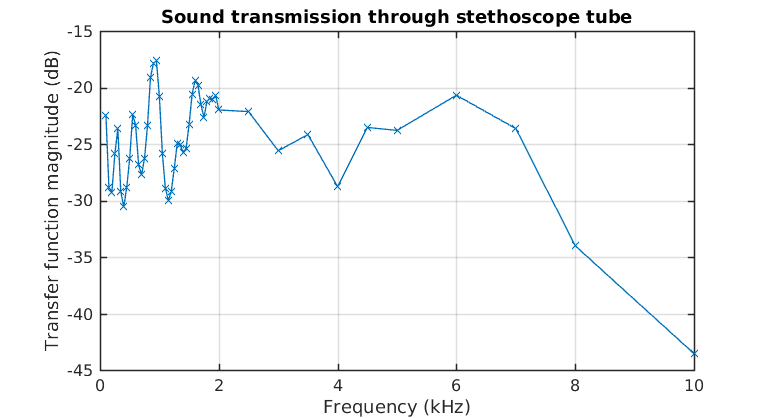
\includegraphics[width=140mm]{result_tubing_freq_response.png}
	 % }
	\caption{Frequency response of sound travelling through stethoscope tubing}
	\label{fig:result_tubing_freq_response}
\end{figure}

\section{Auscultation Frequencies} \label{max-sound-freq}
In order optimise our system we determine what is the maximum sound frequency $f_{max}$ that it needs to measure. This frequency affects the design of the low pass filter and the sampling frequency needed for Analog to Digital Conversion. A lower $f_{max}$ results in a lower sampling frequency, which allows the microprocessor to carry out more computations per sample, and thus allows for higher order digital filters to be implemented. Higher order filters give greater flexibility in digitally manipulating the sound signal, and so would allow us to more accurately reproduce the sound characteristics of a conventional stethoscope.

An $f_{max}$ of 20kHz has been used in our design as this is the threshold of human hearing\cite[p.~163]{Stuart2011}, however it has been stated that the majority of heart and lung sounds occur at lower frequencies, within the range 37.5-1,000 Hz\cite{Abella1992}. In order to determine a lower limit on $f_{max}$ one hundred heart and lung sounds were analysed for their spectral content. Sound files were taken from an electronic resource used to train medical students in auscultation\cite{Coviello2014}, and three analyses were performed using MATLAB. 

The first analysis simply took a Fast Fourier Transform (FFT) of the sounds, summed the amplitudes and defined $f_{max}$ as the frequency at which this sum dropped below -80dB. In the second analysis all the sound signals were summed together, an FFT was performed on the resulting signal, and $f_{max}$ was defined to be the frequency at which the amplitude dropped below -80dB. In the third analysis the significant frequency components of each sound was calculated. Significant frequencies were defined as the range which contained 99.9\% of the signal energy, where energy is the sum of the squared FFT amplitudes. To calculate significant frequencies an iterative algorithm was used. The algorithm begins with a set that contains the signal's dominant frequency, it then adds to this set the next highest or lowest frequency, which ever has the larger FFT amplitude. The energy content of the set is compared with the energy of the sound, and the process continues until the set contains at least 99.9\% of the energy. Finally we took $f_{max}$ to be the largest frequency with at least one sound in which $f_{max}$ was considered significant. 

Analysis 1, 2, and 3 gave $f_{max}$ values 1.9kHz, 1.6kHz, and 4.0kHz respectively (Fig~\ref{fig:ausc_spectra}). If we use the most conservative result then our stethoscope needs to be able to measure and process frequencies up to at least 4.0kHz in order to capture all heart and lung sounds.

\begin{figure}[htb]
	\centering
	 \fbox{
		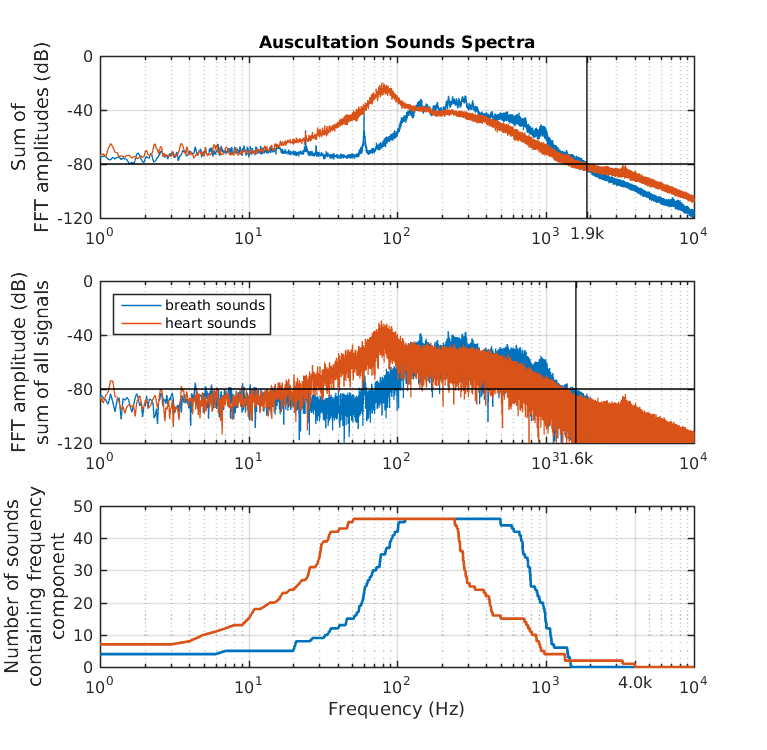
\includegraphics[width=135mm]{auscultation_spectra.png}
	 }
	\caption{Frequency spectra of auscultation sounds}
	\label{fig:ausc_spectra}
\end{figure}



